\chapter{Implementacija i korisničko sučelje}
		
		
		\section{Korištene tehnologije i alati}
		
			\indent \indent Komunikacija grupe se odvijala putem aplikacije \href{https://www.whatsapp.com/}{WhatsApp\footnote{https://www.whatsapp.com/}}, dok je za održavanje sastanaka na daljinu korištena aplikacija \href{https://www.microsoft.com/en-us/microsoft-teams/group-chat-software/}{MicrosoftTeams\footnote{https://www.microsoft.com/en-us/microsoft-teams/group-chat-software/}}, koja pruža opciju video poziva. Sustav \href{https://git-scm.com/}{Git\footnote{https://git-scm.com/}} je omogućio upravljanje različitim verzijama programskog koda i dokumentacije uz udaljeni repozitorij na web platformi \href{https://github.com/}{GitHub\footnote{https://github.com/}}. Dokumentacija je pisana u programskom jeziku \href{https://www.latex-project.org/}{LaTeX\footnote{https://www.latex-project.org/}}, a za izradu UML dijagrama korišten je alat \href{https://astah.net/products/astah-uml/}{Astah UML\footnote{https://astah.net/products/astah-uml/}} sa studentskom licencom.
				
			\indent Korištena je kombinacija razvojnih okruženja ovisno o developeru. Aplikacija je napisana koristeći \href{https://eclipseide.org/}{Eclipse IDE\footnote{https://eclipseide.org/}} i \href{https://www.jetbrains.com/idea/}{IntelliJ IDEA\footnote{https://www.jetbrains.com/idea/}}, dok je za pisanje dokumentacije korišteno razvojno okruženje \href{https://code.visualstudio.com/}{Visual Studio Code\footnote{https://code.visualstudio.com/}}. Eclipse je \textit{open-source} integrirano razvojno okruženje koje se dominantno koristi za razvoj Java aplikacija uz Java razvojne alate. Moguće je prilagoditi okruženje za razvoj web-stranica, web-aplikacija i mobilnih aplikacija uz alate za razvoj programskih aplikacija. Intellij IDEA je integrirano razvojno okruženje tvrtke JetBrains za razvoj računalnih programa u Javi, Kotlinu te drugim programskim jezicima koji se oslanjaju na Java virtualni stroj. Sadrži brojne značajke koje znatno olakšavaju pisanje aplikacija kao što su posebni alati za radne okvire Spring i Spring Boot, pametno popunjavanje koda i podrška pri radu s HTTP porukama. Visual Studio Code je integrirano razvojno okruženje tvrtke Microsoft koje se koristi za razvoj računalnih programa u brojnim računalnim jezicima poput Python, C/C++ i Java. Sva korištena razvojna okruženja su podržana na operacijskim sustavima Microsoft, Linux i macOS. \\
				
			\indent Aplikacija je napravljena u radnom okviru \href{https://spring.io/projects/spring-boot/}{Spring Boot\footnote{https://spring.io/projects/spring-boot/}} kao \href{https://maven.apache.org/}{Maven\footnote{https://maven.apache.org/}} projekt. Za izradu \textit{backenda} aplikacije korišten je programski jezik \href{https://www.java.com/en/}{Java\footnote{https://www.java.com/en/}}, a za izradu \textit{frontenda} je korišten \href{https://react.dev/}{React\footnote{https://react.dev/}} i programski jezik \href{https://www.javascript.com/}{JavaScript\footnote{https://www.javascript.com/}}. Spring Boot je specijalizacija radnog okvira Spring koji se temelji na višeslojnoj arhitekturi čiji je cilj ubrzati i pojednostaviti razvoj web-aplikacija. Spring boot pruža podršku za automatsko definiranje programskih zahtjeva prilikom stvaranja projekata, za ugrađeni server Tomcat i za bazu podataka. Maven je programska podrška za organizaciju projekata i automatizaciju pokretanja aplikacija. Koristimo \textit{in-memory} \href{https://www.h2database.com/html/main.html}{H2\footnote{https://www.h2database.com/html/main.html}} bazu podataka koju pruža Spring Boot. React je biblioteka u JavaScriptu za izgradnju korisničkih sučelja temeljenih na komponentama koju održava Facebook. Glavne značajke React-a su ponovno korištenje web komponenti i ponovno prikazivanje samo komponente koje su promijenjene, a ne cijelu stranicu. Uspostava sobe za video poziv je omogućena preko \href{https://www.daily.co/}{Daily\footnote{https://www.daily.co/}} WebRTC usluga. Ispitivanje projekta je provedeno pomoću \href{https://www.selenium.dev/documentation/webdriver/}{Selenium WebDriver\footnote{https://www.selenium.dev/documentation/webdriver/}}.

		\eject 
		
	
		\section{Ispitivanje programskog rješenja}
			
			\textbf{\textit{dio 2. revizije}}\\
			
			 \textit{U ovom poglavlju je potrebno opisati provedbu ispitivanja implementiranih funkcionalnosti na razini komponenti i na razini cijelog sustava s prikazom odabranih ispitnih slučajeva. Studenti trebaju ispitati temeljnu funkcionalnost i rubne uvjete.}
	
			
			\subsection{Ispitivanje komponenti}
			\textit{Potrebno je provesti ispitivanje jedinica (engl. unit testing) nad razredima koji implementiraju temeljne funkcionalnosti. Razraditi \textbf{minimalno 6 ispitnih slučajeva} u kojima će se ispitati redovni slučajevi, rubni uvjeti te izazivanje pogreške (engl. exception throwing). Poželjno je stvoriti i ispitni slučaj koji koristi funkcionalnosti koje nisu implementirane. Potrebno je priložiti izvorni kôd svih ispitnih slučajeva te prikaz rezultata izvođenja ispita u razvojnom okruženju (prolaz/pad ispita). }
			
			
			
			\subsection{Ispitivanje sustava}
			
			 \textit{Potrebno je provesti i opisati ispitivanje sustava koristeći radni okvir Selenium\footnote{\url{https://www.seleniumhq.org/}}. Razraditi \textbf{minimalno 4 ispitna slučaja} u kojima će se ispitati redovni slučajevi, rubni uvjeti te poziv funkcionalnosti koja nije implementirana/izaziva pogrešku kako bi se vidjelo na koji način sustav reagira kada nešto nije u potpunosti ostvareno. Ispitni slučaj se treba sastojati od ulaza (npr. korisničko ime i lozinka), očekivanog izlaza ili rezultata, koraka ispitivanja i dobivenog izlaza ili rezultata.\\ }
			 
			 \textit{Izradu ispitnih slučajeva pomoću radnog okvira Selenium moguće je provesti pomoću jednog od sljedeća dva alata:}
			 \begin{itemize}
			 	\item \textit{dodatak za preglednik \textbf{Selenium IDE} - snimanje korisnikovih akcija radi automatskog ponavljanja ispita	}
			 	\item \textit{\textbf{Selenium WebDriver} - podrška za pisanje ispita u jezicima Java, C\#, PHP koristeći posebno programsko sučelje.}
			 \end{itemize}
		 	\textit{Detalji o korištenju alata Selenium bit će prikazani na posebnom predavanju tijekom semestra.}
			
			\eject 
		
		
		\section{Dijagram razmještaja}
			
			%\textbf{\textit{dio 2. revizije}}
			
			 %\textit{Potrebno je umetnuti \textbf{specifikacijski} dijagram razmještaja i opisati ga. Moguće je umjesto specifikacijskog dijagrama razmještaja umetnuti dijagram razmještaja instanci, pod uvjetom da taj dijagram bolje opisuje neki važniji dio sustava.}
			 Dijagramom razmještaja opisuje se topologija sustava i odnos različitih sklopovskih i programskih komponenti sustava. Sustav je temeljen na arhitekturi klijent-poslužitelj, a sastoji se od dva poslužiteljska računala. Na prvom se poslužitelju u okruženju NodeJS pokreće front-end aplikacije. Klijenti uz pomoć internetskog preglednika pristupaju aplikacije preko front-enda korištenjem protokola HTTP.
			 
			 Front-end će po potrebi proslijediti HTTP zahtjev drugom poslužitelju na kojem se nalaze back-end aplikacije i baza podataka koji se radi jednostavnosti i prenosivosti pokreću u Docker kontejneru. Kada dobije HTTP zahtjev od front-enda, back-end bazi podataka šalje odgovarajući upit, a nakon što dobije odgovor, šalje ga front-endu koji ga onda koristi kako bi odgovorio klijentu.
			\begin{figure}[H]
				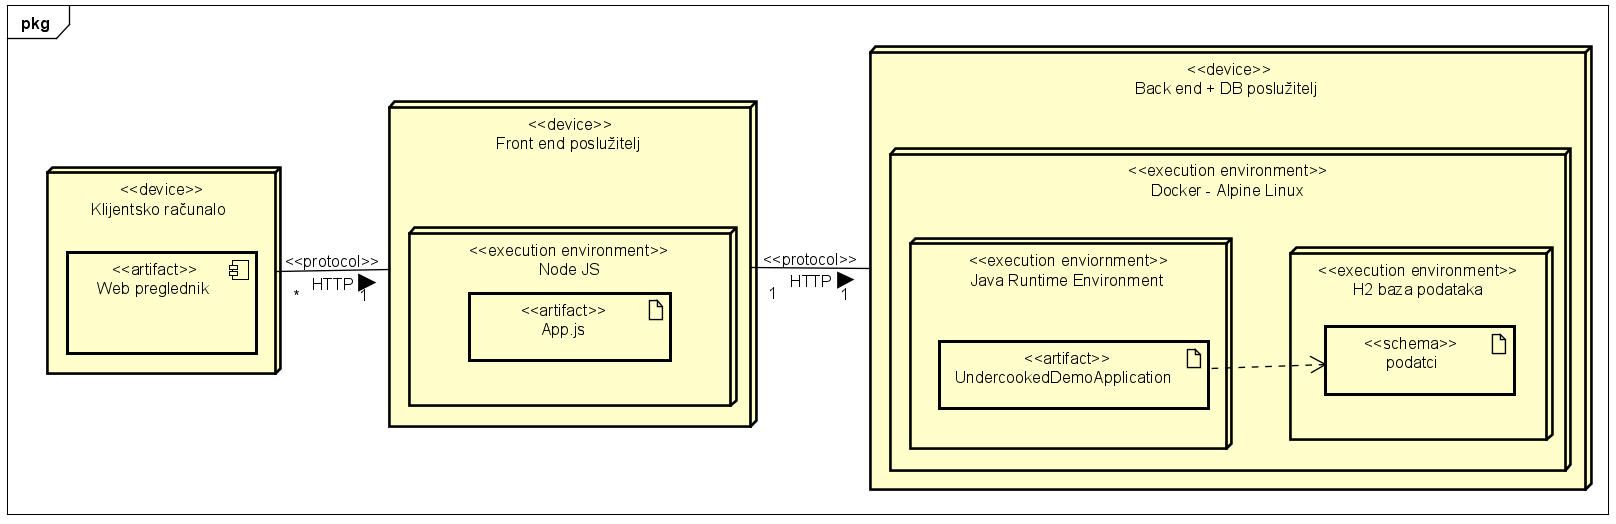
\includegraphics[scale=0.35]{slike/dijagram_razmjestaja.png} %veličina slike u odnosu na originalnu datoteku i pozicija slike
				\centering
				\caption{Dijagram razmještaja}
				\label{fig:Dijagram razmještaja}
			\end{figure}
			\eject 
		
		\section{Upute za puštanje u pogon}
		
			\textbf{\textit{dio 2. revizije}}\\
		
			 \textit{U ovom poglavlju potrebno je dati upute za puštanje u pogon (engl. deployment) ostvarene aplikacije. Na primjer, za web aplikacije, opisati postupak kojim se od izvornog kôda dolazi do potpuno postavljene baze podataka i poslužitelja koji odgovara na upite korisnika. Za mobilnu aplikaciju, postupak kojim se aplikacija izgradi, te postavi na neku od trgovina. Za stolnu (engl. desktop) aplikaciju, postupak kojim se aplikacija instalira na računalo. Ukoliko mobilne i stolne aplikacije komuniciraju s poslužiteljem i/ili bazom podataka, opisati i postupak njihovog postavljanja. Pri izradi uputa preporučuje se \textbf{naglasiti korake instalacije uporabom natuknica} te koristiti što je više moguće \textbf{slike ekrana} (engl. screenshots) kako bi upute bile jasne i jednostavne za slijediti.}
			
			
			 \textit{Dovršenu aplikaciju potrebno je pokrenuti na javno dostupnom poslužitelju. Studentima se preporuča korištenje neke od sljedećih besplatnih usluga: \href{https://aws.amazon.com/}{Amazon AWS}, \href{https://azure.microsoft.com/en-us/}{Microsoft Azure} ili \href{https://www.heroku.com/}{Heroku}. Mobilne aplikacije trebaju biti objavljene na F-Droid, Google Play ili Amazon App trgovini.}
			
			
			\eject 